\chapter{\IfLanguageName{dutch}{Proof of Concept}{Proof of Concept}}%
\label{ch:poc}

\section{\IfLanguageName{dutch}{Applicatie Ontwerp}{Application Design}}%
\label{sec:design}

For this proof-of-concept example a simple functionality will be implemented. User should be able to make measurements notes (logs) inside custom defined tables (logbooks). Each row contains a 'moment' field representing date and time of a measurement, up to 4 numeric fields representing values and a comment field. Some default predefined logbooks with most common body parameters will be added. Currently displayed lobkook will be chosen by selecting a button at the top of the page. If all logbooks do not fit inside the bar, two arrows will appear to allow scrolling left and right.

\begin{figure}[H]
    \centering
    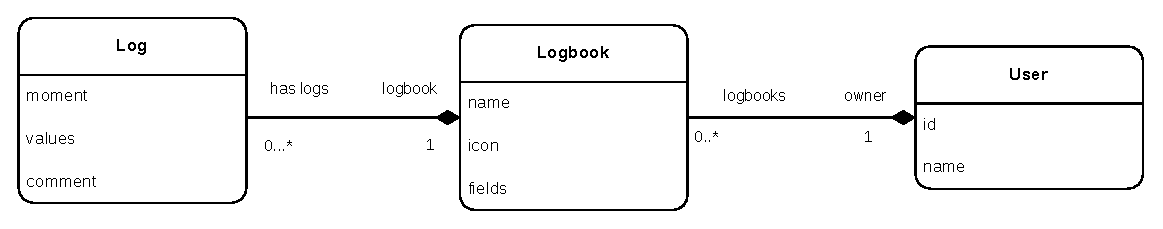
\includegraphics[width=0.8\textwidth]{conceptual-model.eps}
    \caption[Conceptual Model Diagram]{\label{fig:conceptmodel} Conceptual Model Diagram of the application}
\end{figure}

\begin{figure}[H]
    \centering
    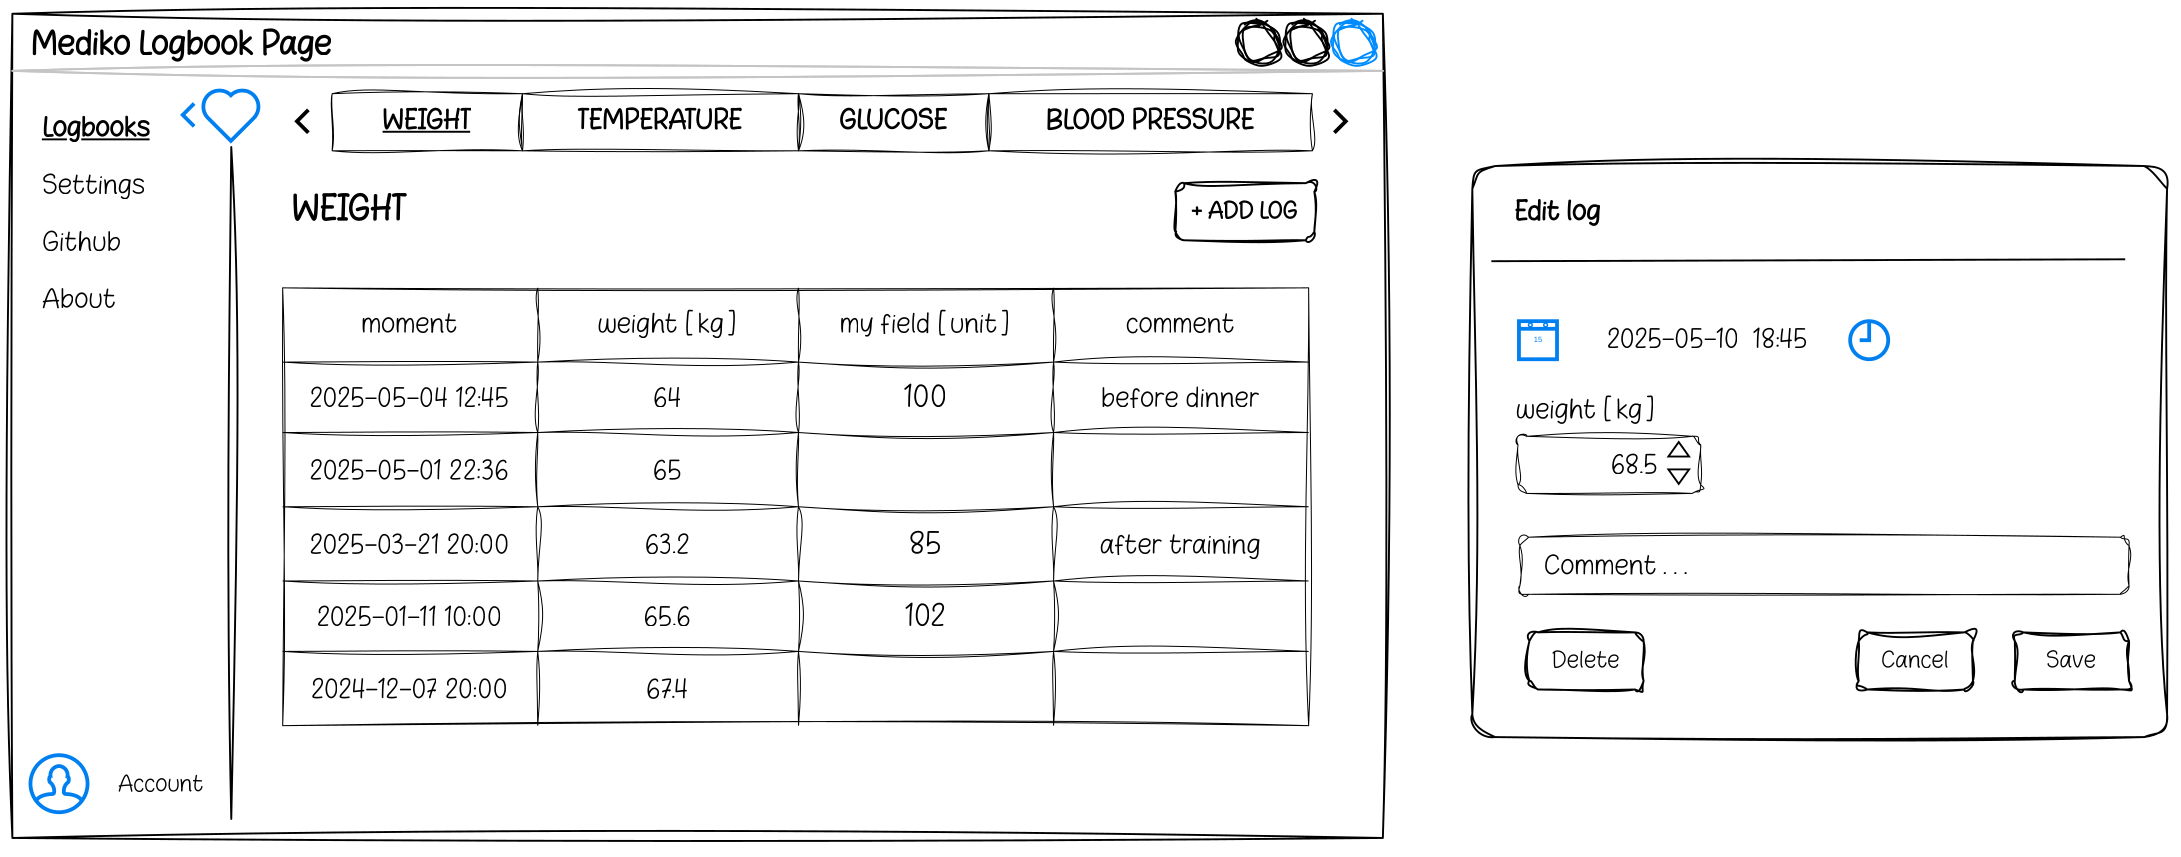
\includegraphics[width=0.8\textwidth]{layout-logbook.png}
    \caption[Logbooks page layout design]{\label{fig:layoutlogbook} Layout design of the logbooks page. Logbook Table (left), log edit menu (right) }
\end{figure}

On the Settings page user will be able to edit, remove and also create own custom logbooks with specified fields, units and (optionally) value precision. Before each line a checkbox will determine which logbooks should be visible on the tabs-bar on the logbooks page. Before  deletion of a logbook, an confirmation dialog must be shown.

\begin{figure}[H]
    \centering
    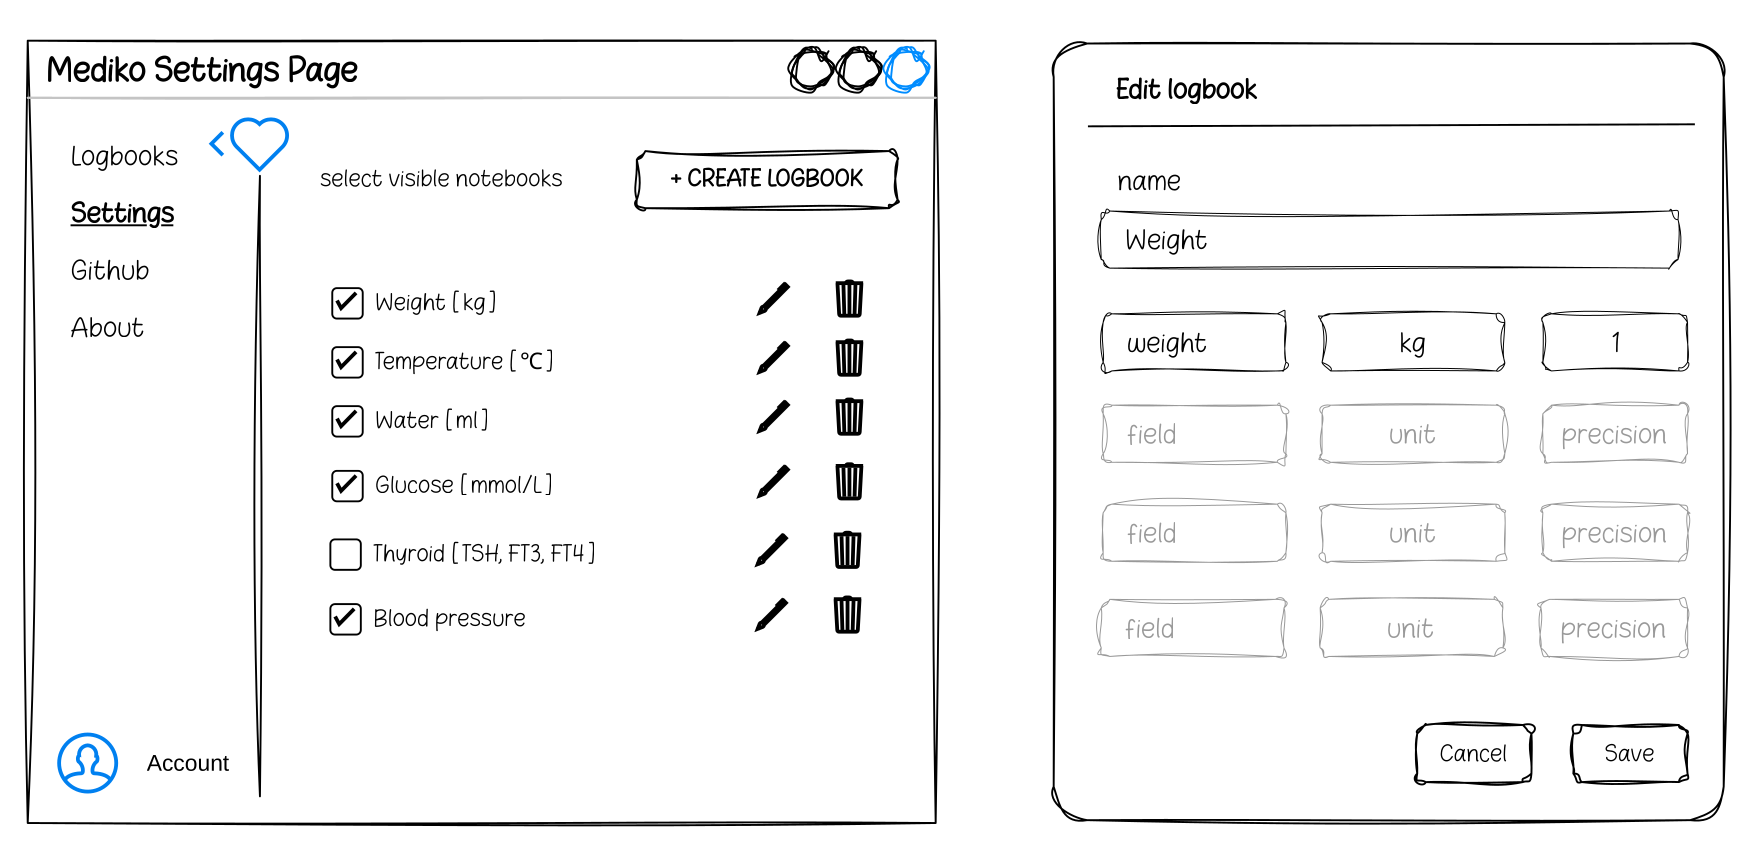
\includegraphics[width=0.8\textwidth]{layout-settings.png}
    \caption[Settings page layout design]{\label{fig:layoutsettings} Layout design: Settings page with available logbooks (left), logbook edit menu (right)}
\end{figure}

To achieve the greatest flexibility, client-server architecture will be used. One of the biggest advantages of this solution is the ability to share information resources among different users or devices belonging to the same user. In other words, data consistency is improved, what ensures all clients access the latest data from a one central source, minimizing divergences. Moreover centralized data storage allows for effective backups and management, enhancing data reliability. There is also possibility for errors isolation - client applications failures do not affect the server or other clients, what improves overall system stability making maintanace easier.
The intention is to allow the application to work completely in offline mode, and synchronize the locally saved data with the cloud server, at the user's request or automatically in the background. 

\begin{figure}[H]
    \centering
    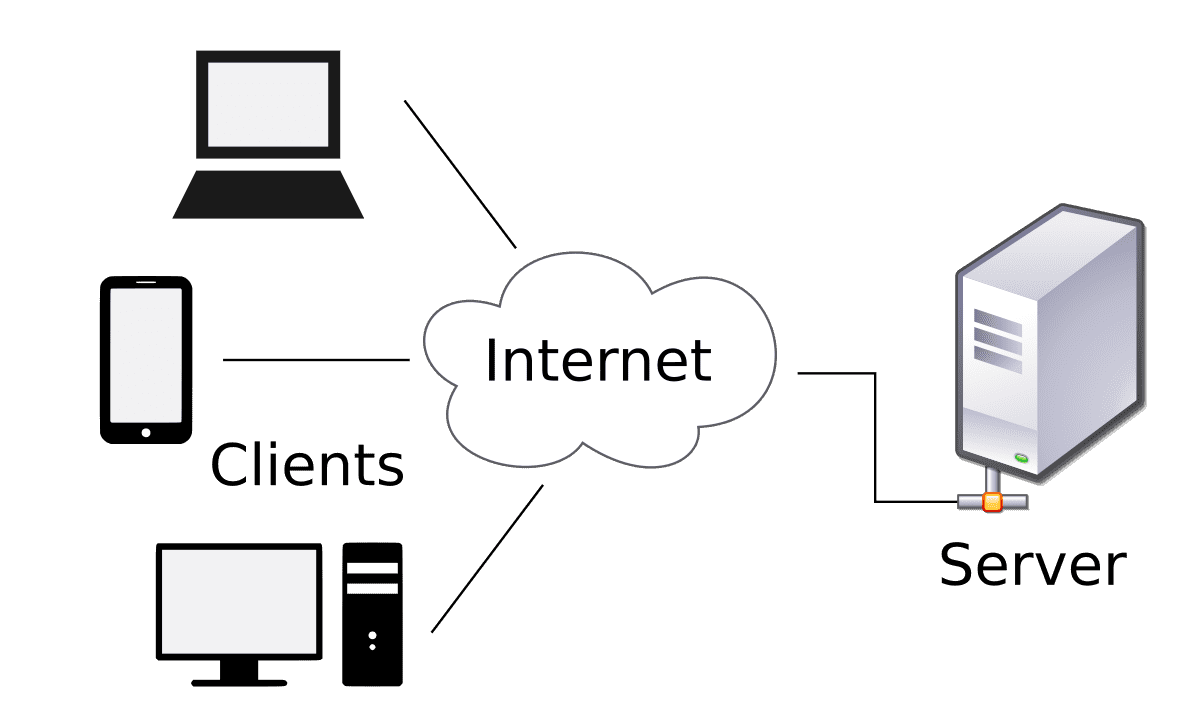
\includegraphics[width=0.8\textwidth]{client-server-architecture.png}
    \caption[Solution Architecture]{\label{fig:architecture} Solution client-server architecture }
\end{figure}

 

\section{{Language and framework choice}}

After a detailed analysis of the available solutions for writing the code, JavaScript was selected (or more precisely its extended variant - TypeScript). Below are the point arguments:

\begin{itemize}
  \item \textbf{Great popularity:} JavaScript seems to be the most widespread language across all devices types.
  \item \textbf{Wide range of available libraries and frameworks:} There are many popular JS libraries and frameworks available (mostly open-source) that can help implement desired functionalities.
  \item \textbf{Acceptable performance:} JavaScript uses so called Just-in-Time Compiler technique (JIT)\autocite{JIT}. At the runtime it's not the fastest language but unlike compiled languages (like for example C++) where the source code is converted into machine code before execution, it doesn't take much time to start up after making changes to the code because it doesn't need to go through that compilation step at the beginning.
\end{itemize}

To improve implementation of Object-Oriented Programming principles (OOP) both client and server will be written in TypeScript, a developed by Microsoft superset of JavaScript that adds optional static typing and other features to the language. TypeScript is compiled/transpiled into JavaScript, ensuring it works in all JS environments. Using TS can provide several advantages over plain JS, including:
\begin{itemize}
    \item \textbf{Static typing} allows programmers to define variable types and helps catch errors before running the code. It also improves quality and readability of the code.
    \item \textbf{Extra features} like generics, mapped types, utility-, intersection-, union- and conditional types, interfaces
    \item \textbf{Better Scalability:} TypeScript is used to manage and grow large projects. It makes it easier to maintain complex codebases over time.
\end{itemize}
\autocite{TSDoc} \autocite{TSfeatures}
\newline

Vue.js is one of the three most popular JavaScript framework (next to Angular, React) for building user  interfaces. It provides a declarative, component-based programming model that helps develop user interfaces of any complexity \autocite{VueDoc}. According to the official documentation Vue.js has two most important core features:
\begin{itemize}
    \item \textbf{Declarative Rendering:} Vue extends standard HTML with a template syntax that allows developers to declaratively describe HTML output based on JavaScript state.
    \item \textbf{Reactivity:} Vue automatically tracks JavaScript state changes and efficiently updates the DOM when changes happen.
\end{itemize}


Programmers can choose between two coding styles:
\begin{itemize}
    \item \textbf{Options API} is the traditional method of building Vue components and has been a core feature of Vue since its inception. The Options API in Vue organizes component logic into clearly defined options like data, methods, and computed, offering a familiar and structured approach to managing component behavior.
    \item \textbf{Composition API} is a newer way of building components in Vue since version 3 that was introduced to address some of the limitations of the Options API. The Composition API in Vue allows developers to use a functional, reactive programming style to build components, and it offers a more flexible and expressive way of defining component behavior.
\end{itemize}
Each approach brings its own set of advantages and challenges, making the decision on which one to use a critical consideration for any project. In this thesis for the proof-of-concept project the newer Composition API will be used.

\begin{listing}[H]
    \begin{minted}{vue}
    <template>
        <div>
            <p>{{ props.title }}</p>
            <p @click="increment">Clicks: {{ clickCount }}</p>
        </div>
    </template>
    
    <script setup lang="ts">
    import { Ref, ref } from "vue";
    interface ExampleProps {
        title: string;
    }
    const props = defineProps<ExampleProps>();
    const clickCount: Ref<number> = ref(0);
    function increment() {
        clickCount.value += 1;
        return clickCount.value;
    }
    </script>
    
    <style lang="css">
    p {
        color: red;
    }
    </style>
    \end{minted}
\caption[Vue document example]{Example of .vue document including 3 sections: \newline <template> : where html document structure is defined, \newline<script> : with example TypeScript code, \newline<style> : containing CSS style for current component}
\end{listing}

Quasar is an an MIT licensed open-source js framework build on top of the Vue.js using its reactivity and component-based architecture. It offers a wide range of customizable pre-built UI components (such as buttons, forms, tables, infinite scrolling, dialogs, notifications, etc...) allowing developers to focus on implementing functionalities. Quasar has built-in support for responsive and mobile-first design. Its biggest benefit is the availability of all features in one place, accessible from the CLI level and online documentation.
Through the CLI built-in functions framework allows to test and deploy once written code simultaneously as a website, a Mobile App and/or an standalone Desktop Application. \autocite{QuasarStart}

\section{\IfLanguageName{dutch}{Voorbereiding}{Prerequisites}}%
\label{sec:prerequisites}

The software is being developed on a PC machine with x64 architecture running Fedora Linux. The project  will be managed on the Azure DevOps where tasks are described and issues tracked. GitHub repository was initialized for code version control and cloned locally. The machine has already installed Node.js - a JavaScript runtime environment, Node Package Manager \autocite{npm} and Node Version Manager \autocite{nvm}. 

Quasar framework provides own command line interface (CLI) allowing access to more features and automating some tasks. The CLI will be installed globally to make possible to directly run Quasar commands in the terminal, run a local http server for testing or do upgrades on the project \autocite{QuasarStart}. According to the Quasar documentation, the following code needs to be executed:

\begin{verbatim}
    npm i -g @quasar/cli

\end{verbatim}

\section{\IfLanguageName{dutch}{Installatie}{Client Template Installation}}%
\label{sec:installation}

New Quasar project is initialised with the command:
\begin{verbatim}
    npm init quasar@latest

\end{verbatim}

Installation wizard asks some questions about preferences to automatically generate startup project template. The developer chooses first a project type (in most cases it's an application) and folder name. Command is executed inside already initialised git repo, so folder 'client' becomes a subfolder of the whole project repository. 

\begin{verbatim}
? What would you like to build? > - Use arrow-keys. Return to submit.
>  App with Quasar CLI, let's go! - spa/pwa/ssr/bex/electron/capacitor/cordova
   AppExtension (AE) for Quasar CLI
   Quasar UI kit
   
? Project folder: > client

\end{verbatim}

The next question is about choosing the project language. For better support of the OOP paradigm, it is recommended to choose TypeScript, which extends JavaScript, among others, the possibility of type declaration \autocite{TSDoc}
\begin{verbatim}
    ? Pick script type: >
        Javascript
    >   Typescript

\end{verbatim}

The default and recommended by Vue.js and Quasar local UI development server is Vite including a Hot Module Replacement (HMR) system, which works by just reloading the specific file being changed instead of recompiling the entire application \autocite{Vite}. 
\begin{verbatim}
    ? Pick Quasar App CLI variant: >
    >   Quasar App CLI with Vite - recommended
        Quasar App CLI with Webpack

\end{verbatim}    

Vue.js comes with two programmings styles, the newer one - Composition API is recommended because of better TypeScript support \autocite{VueAPIStyles}
% add reference to detailed description
\begin{verbatim}
    ? Pick a Vue component style: > 
    >   Composition API with <script setup> - recommended
        Composition API
        Options API

\end{verbatim}

\begin{verbatim}
    ? Pick your CSS preprocessor: > 
    >   Sass with SCSS syntax
        Sass with indented syntax
        None (the others will still be available)
\end{verbatim}

Additional package(s) suggested by the CLI, in this case Pinia State Management and Axios (promise based HTTP client for the web-browser and node.js) are choosen.
% add reference to detailed description
\begin{verbatim}
    ? Check the features needed for your project: >  
    ◯   Linting (vite-plugin-checker + ESLint + vue-tsc)
    ◉   State Management (Pinia)
    ◉   axios
    ◯   vue-i18n
    
    Quasar •  SUCCESS  • The project has been scaffolded

    ? Install project dependencies? (recommended)
    >   Yes, use npm
        No, I will handle that myself 

\end{verbatim}
    

Quasar CLI shows the summary of choosen options:

\begin{verbatim}
What would you like to build? > App with Quasar CLI, let's go!
Project folder: … client
Pick script type: > Typescript
Pick Quasar App CLI variant: > Quasar App CLI with Vite
Package name: … mediko-client
Project product name: > … Mediko
Project description: > … Cross-platform application with Vue, Quasar
Pick a Vue component style: > Composition API with <script setup>
Pick your CSS preprocessor: > Sass with SCSS syntax
Check the features needed for your project: > State Management (Pinia), axios
\end{verbatim}

\section{\IfLanguageName{dutch}{Web client applicatie}{Single Page Application Web Client}}%
\label{sec:webclient}

To start the web application in browser with Quasar CLI we need to navigate to the client folder and call Quasar CLI dev command.

\begin{verbatim}
    cd client
    quasar dev
\end{verbatim}

The template is now working - project startup applications automatically opens in default browser:

\begin{figure} [H]
    \centering
    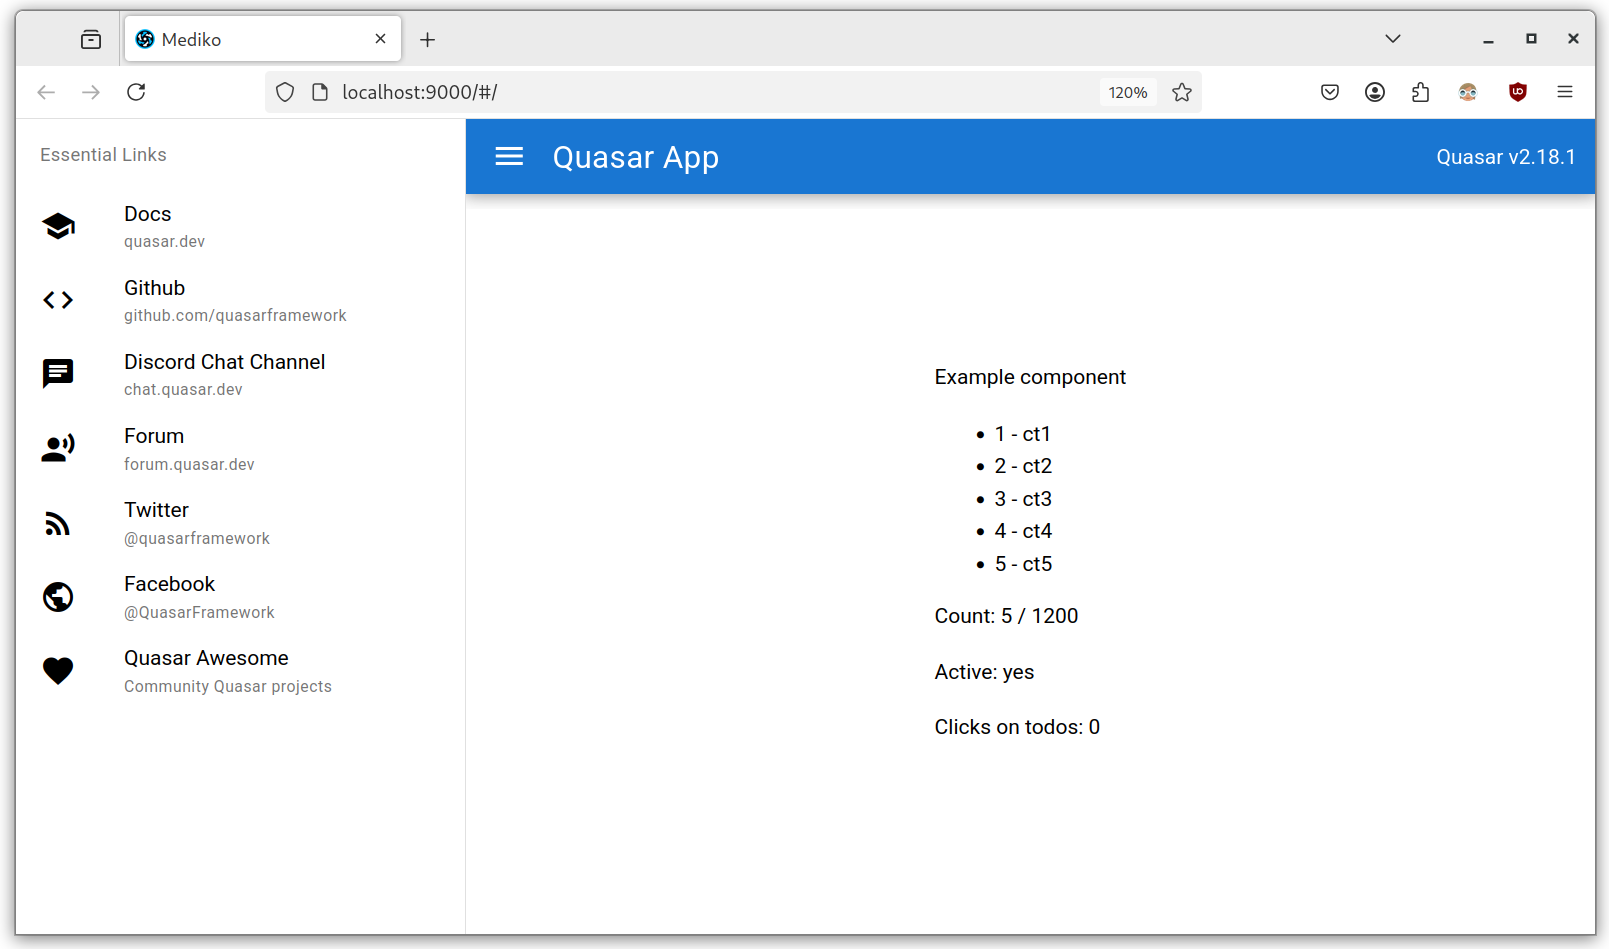
\includegraphics[width=0.8\textwidth]{templ-layout.png}
    \caption[Client Template]{\label{fig:template}Created Project template in the web browser.}
\end{figure}

Initially, the project contains an example clicks-counter and some Quasar related navigation links in the drawer, they will be removed in the next step to prepare template for implementations of proof-of-concept functionalities.


\section{{Implementation of Functionalities}}%
\label{sec:functionalities}
% Logbooks, log, edit logs, 
% class diagram
% Local Storage

In the first step, entity models were created in apart folder (Logbook and Log). They both inherit properties from abstract class TrackedEntity, which contains identity property as uuid (128-bit values that are canonically represented as a 36-character string in the format 123e4567-e89b-12d3-a456-426614174000, 5 hex strings separated by hyphens) string \autocite{UUID}, it allows multiple clients independently create items without conflict during synchronization.

\begin{listing}[H]
    \begin{minted}{ts}
    import { v4 as uuidv4 } from 'uuid';
    export class TrackedEntity {
        id: string = uuidv4();
        createdAt?: Date;
        updatedAt?: Date;
        deletedAt?: Date | null = null;
        isDeleted?: boolean = false;
    }
    \end{minted}
\caption[Tracked Entity]{Abstract TrackedEntity inherited by Mediko Entity classes Log, Logbook}
\end{listing}


The client application design model is described by the diagram below:

\begin{figure}[H]
    \centering
    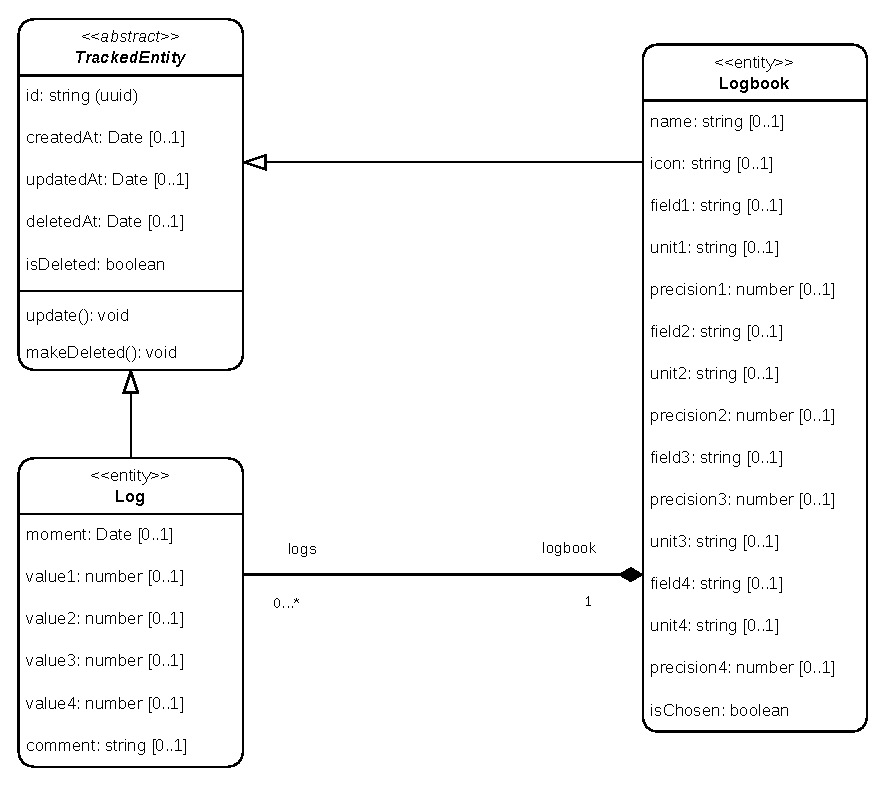
\includegraphics[width=0.8\textwidth]{info-design-model.eps}
    \caption[Class Diagram]{\label{fig:infomodeldiagram} Client App Information Design Model Class Diagram }
\end{figure}

Data management methods are seperated from the model view logic and placed in apart service class  (LogbookLocalService). Mediko has to work independently as standalone application, so data are saved in browser LocalStorage and preserved as long as the browser cache will not be cleared. Quasar framework provides already included wrapper around Web Storage API - mechanisms by which browsers can store key/value pairs \autocite{MozillaLocalStorage}.

\begin{figure}[H]
    \centering
    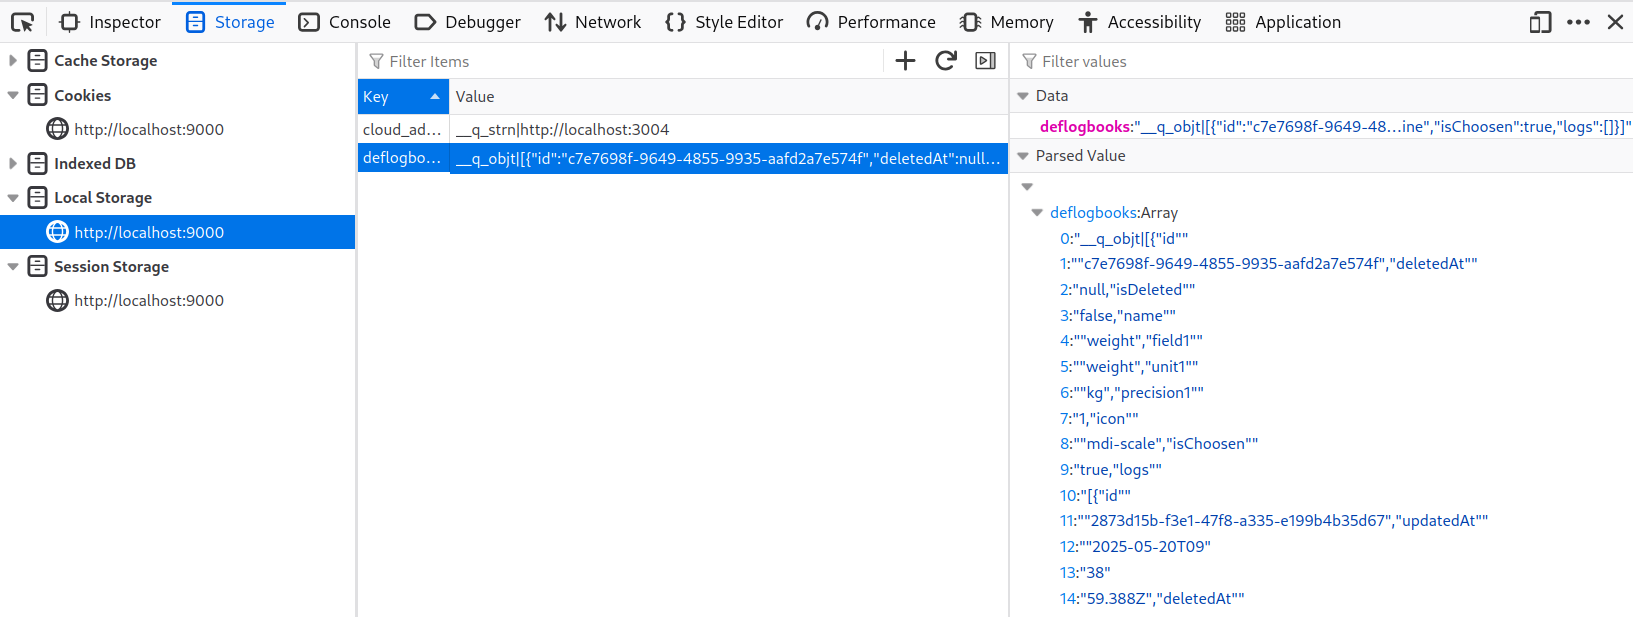
\includegraphics[width=0.8\textwidth]{local-storage.png}
    \caption[LocalStorage]{\label{fig:localstorage} Local Storage in Firefox Dev Tools }
\end{figure}

\begin{figure}[H]
    \centering
    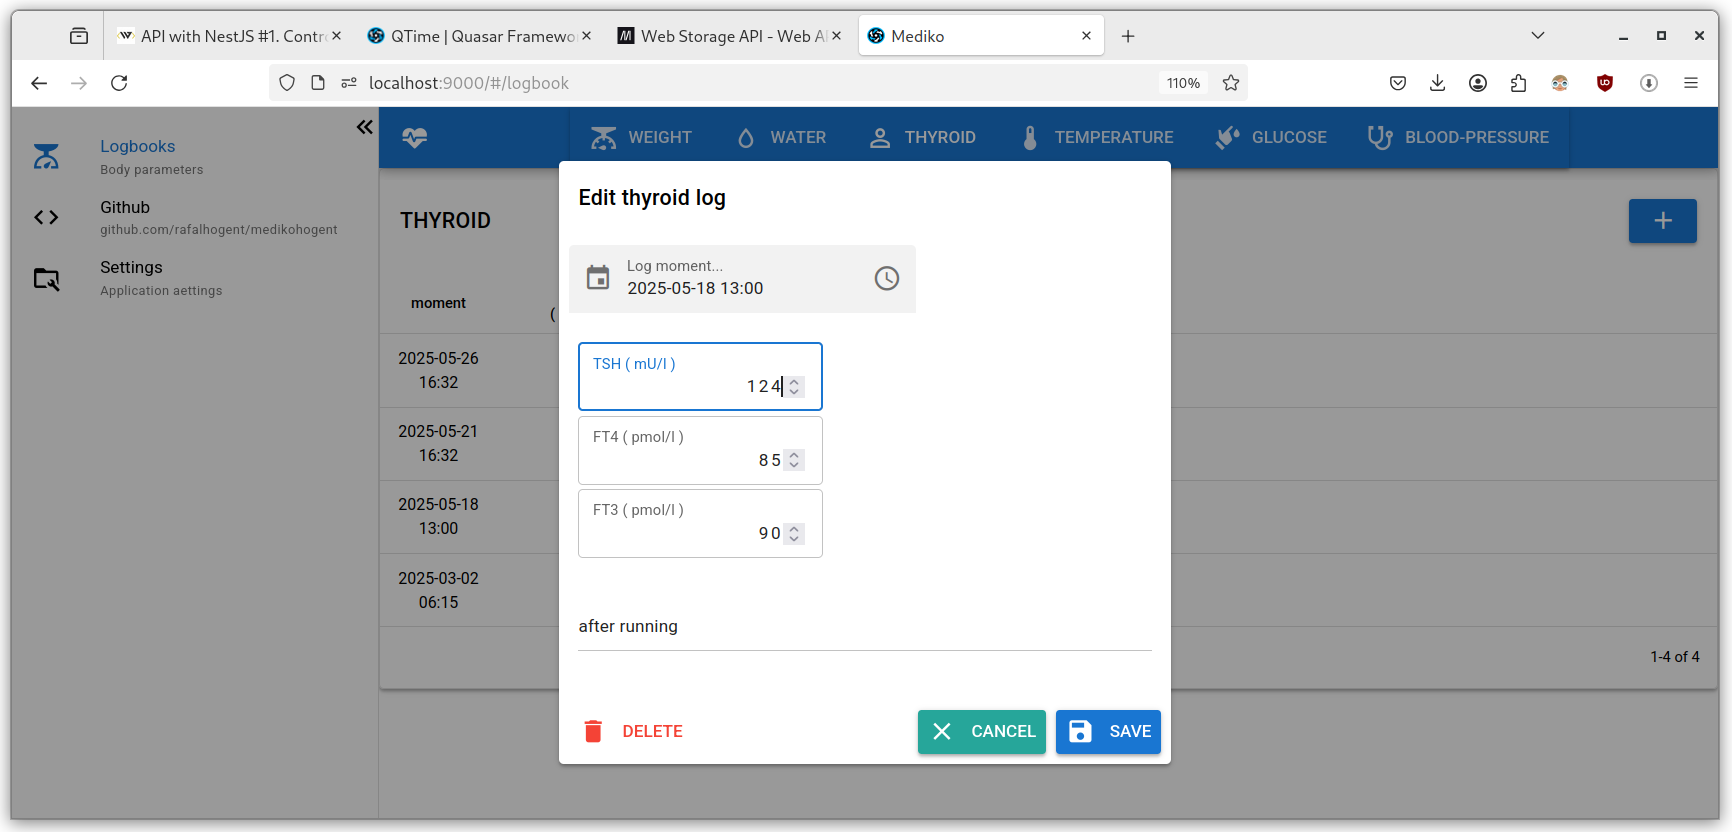
\includegraphics[width=0.7\textwidth]{screen-editlog.png}
    \caption[Editing Log in Web Browser]{\label{fig:editlogs} Mediko web application running in web browser. Editing logs menu }
\end{figure}


\begin{figure}[H]
    \centering
    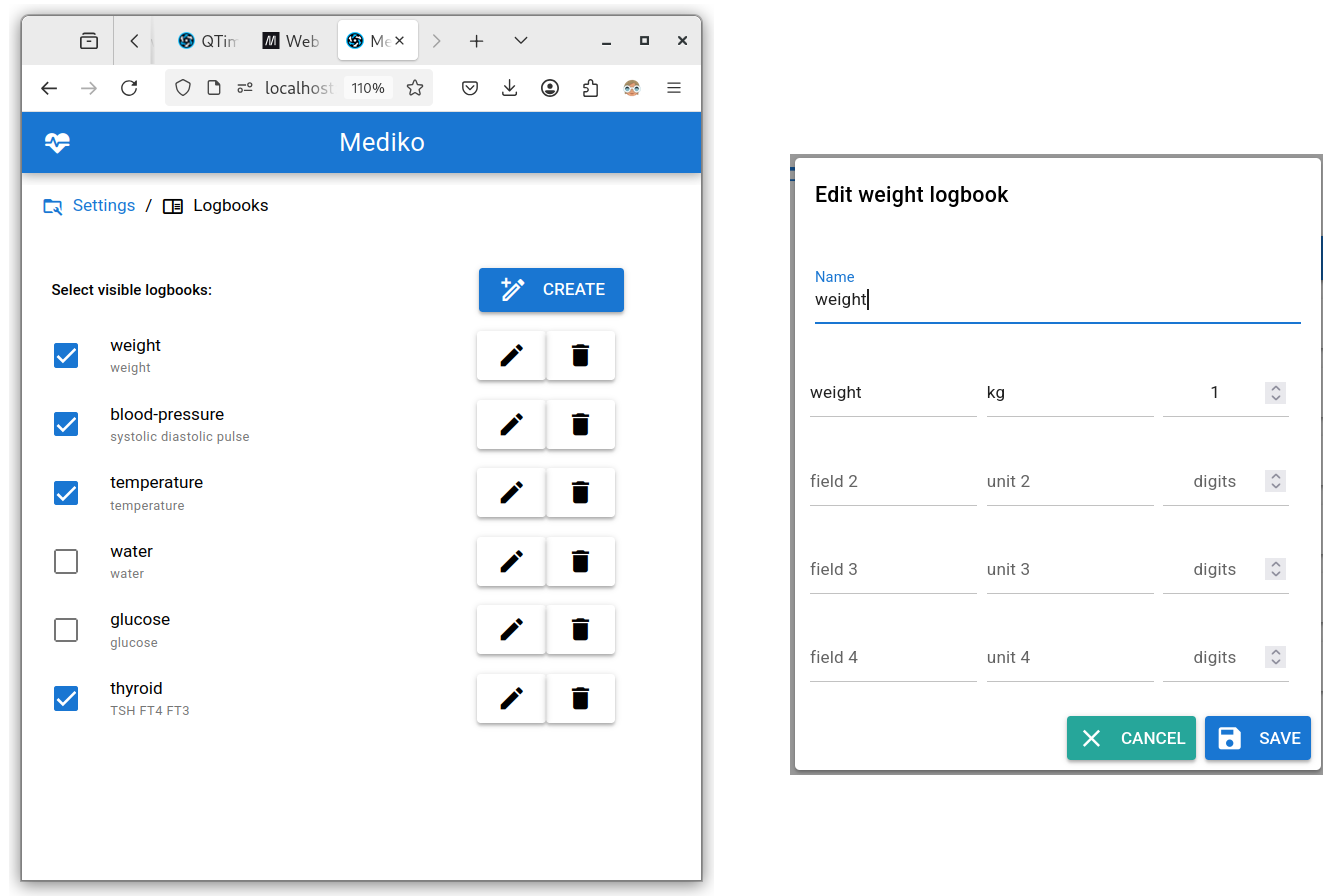
\includegraphics[width=0.7\textwidth]{screen-settings.png}
    \caption[Screen settings]{\label{fig:settings} Screen settings and editing logbooks. }
\end{figure}

    

\begin{listing}[H]
    \begin{minted}{ts}
import { LocalStorage } from "quasar";
export class LogbookLocalService {
  static getLocalLogbooks(): Logbook[] {
    const localLogbooks = plainToInstance(
      Logbook,
      LocalStorage.getItem(DEF_LOGBOOKS) as any[]
    );
    if (Array.isArray(localLogbooks) && localLogbooks?.length) {
      const deflogbooks = localLogbooks?.filter((lb) => !lb.isDeleted);
      deflogbooks.forEach((lgb) => {
        lgb.logs = lgb.logs
          .filter((l) => !l.isDeleted)
          .map((l) => plainToInstance(Log, l));
        lgb.logs.forEach((l) => {
          if (l.moment) {
            l.moment = DateTime.fromISO(l.moment.toString()).toJSDate();
          }
        });
      });
      return deflogbooks;
    }
    return [];
  }

  static saveLogbooksData(logbooks: Logbook[]) {
    LocalStorage.setItem(DEF_LOGBOOKS, logbooks);
  }
}
    \end{minted}
\caption[Logbook Local Service]{Client local data storage implementation, part of the featured LogbookLocalService class}
\end{listing}



In the application repository client folder is organized in structured subfolders. In the 'pages' folder are located vue files representing pages-components used by vue-router \autocite{VueRouter}. Folder 'models' contains entities and view-models definition in typescript. Folder 'services' contains 'local' subfolder where are located classes responsible for data management in client local storage, later will be added subfolder with classes responsible for external communication (like data synchronization). The full source code is available on the Github repository attached to the thesis.

\begin{listing}[H]
    \begin{minted}{shell}
        client
        ├── src
            ├── App.vue
            ├── assets
            ├── boot
            ├── components
            │   ├── common
            │   │   └── Confirmation.vue
            │   ├── EssentialLink.vue
            │   └── logbook
            │       ├── EditLogbook.vue
            │       └── EditLog.vue
            ├── css
            ├── layouts
            │   └── MainLayout.vue
            ├── models
            │   ├── common
            │   │   └── tracked-entity.ts
            │   └── logbook
            │       ├── logbook.ts
            │       └── log.ts
            ├── pages
            │   ├── ErrorNotFound.vue
            │   ├── IndexPage.vue
            │   ├── LogbookPage.vue
            │   ├── settings-pages
            │   │   ├── LogbooksSettingsPage.vue
            │   │   └── MainSettingsPage.vue
            │   └── SettingsPage.vue
            ├── router
            │   ├── index.ts
            │   └── routes.ts
            ├── services
            │   └── local
            │       ├── local-keys.ts
            │       └── logbook.local.service.ts
            └── stores
                ├── app.store.ts
                └── index.ts
    \end{minted}
\caption[]{Client Repository folder structure tree}
\end{listing}
